%!TEX TS-program = pdflatex
%!TEX TS-options = -shell-escape
\RequirePackage{fix-cm}


\newcommand{\obenlinks}{Übungen zur Vorlesung Informatik I}   % hier Name der Veranstaltung eintragen
\documentclass[%
  paper=a4,
  fontsize=10pt,
  ngerman
  ]{scrartcl}

% Basics für Codierung und Sprache
% ===========================================================
  \usepackage{shellesc}                 % Compiler-Option -shell-escape benutzen!
  \usepackage[final]{graphicx}          % Einbindung von Grafiken
  \usepackage{subcaption}
%  \usepackage[utf8]{inputenc}          % Dateien sind UTF8-codiert
  \usepackage{babel}                    % deutsche Silbentrennung, etc.
  \usepackage[german=quotes]{csquotes}  % deutsche Anführungszeichen mit \enquote{...}
% ===========================================================

% Fonts und Typographie
% ===========================================================
  \usepackage[babel=true,final,tracking=smallcaps]{microtype}
  \DisableLigatures{encoding = T1, family = tt* }   % keine Ligaturen für Monospace-Fonts
% ===========================================================

% Farben
% ===========================================================
  \usepackage[usenames,x11names,final]{xcolor}
% ===========================================================

% Mathe-Pakete und -Einstellungen
% ===========================================================
  \usepackage{mathtools}               % Tools zum Setzen von Formeln
  \usepackage{amssymb}                 % übliche Mathe-Symbole
  \usepackage[bigdelims]{newtxmath}    % moderne Mathe-Font
  \allowdisplaybreaks                  % seitenübergreifende Rechnungen
  \usepackage{bm}                      % math bold font
  \usepackage{wasysym}                 % noch mehr Symbole
% ===========================================================

% TikZ
% ===========================================================
  \usepackage{tikz}
  \usetikzlibrary{arrows,arrows.meta}    % mehr Pfeile!
  \usetikzlibrary{calc}                  % TikZ kann rechnen
  \usetikzlibrary{positioning}
  \tikzset{>=Latex}                      % Standard-Pfeilspitze
% ===========================================================

% Seitenlayout, Kopf-/Fußzeile
% ===========================================================
  \usepackage{scrlayer-scrpage}
  \pagestyle{scrheadings}
  \usepackage[top=5cm, bottom=3cm, left=2.5cm, right=2cm]{geometry}
  \clearscrheadfoot 
  \setheadsepline{0.4pt}                            % Linie in Kopfzeile
  \setfootsepline{0.4pt}                            % Linie in Fußzeile
  \setkomafont{section}{\fontsize{14bp}{18.8bp}\normalfont}  % Schriftart der Section
  \setkomafont{subsection}{\fontsize{12bp}{16bp}\normalfont}                  
  \setkomafont{pagehead}{\textnormal}                 % Schriftart Kopfzeile
  \setkomafont{pagefoot}{\normalfont\footnotesize}  % Schriftart Fußzeile 
  \cfoot{\thepage}                                  % Seitenzahl unten Mitte
  \lohead{\obenlinks}                               % Titel oben links
  \raggedbottom                                     % Flattersatz
  \usepackage{setspace}                             % erweiterte Abstandsoptionen
  \onehalfspacing                                   % Zeilenabstand 1.5-fach
  \setlength{\parindent}{0pt}                       % Einrückung neuer Absätze
  \setlength{\parskip}{0.5\baselineskip}            % Abstand neuer Absätze
% ===========================================================

% Hyperref für Referenzen und Hyperlinks
% ===========================================================
  \usepackage[%
    hidelinks,
    pdfpagelabels,
    bookmarksopen=true,
    bookmarksnumbered=true,
    linkcolor=black,
    urlcolor=SkyBlue2,
    plainpages=false,
    pagebackref,
    citecolor=black,
    hypertexnames=true,
    pdfborderstyle={/S/U},
    linkbordercolor=SkyBlue2,
    colorlinks=false,
    backref=false]{hyperref}
  \hypersetup{final}
% ===========================================================

% Listen und Tabellen
% ===========================================================
  \usepackage{multicol}
  \usepackage[shortlabels]{enumitem}
  \setlist{itemsep=0pt}
  \setlist[enumerate]{font=\sffamily\bfseries}
  \setlist[itemize]{label=$\triangleright$}
  \usepackage{tabularx}
% ===========================================================

% minted
% ===========================================================
\usepackage{minted}
\setminted{%
  style=default,
  fontsize=\small,
  breaklines,
  breakanywhere=false,
  breakbytoken=false,
  breakbytokenanywhere=false,
  breakafter={.,},
  autogobble,
  numbersep=3mm,
  tabsize=4,
  linenos,
  frame=lines
}
\setmintedinline{%
  fontsize=\normalsize,
  numbers=none,
  numbersep=12pt,
  tabsize=4,
}

%%%%%%%%%%%%%%%%%%%%%%%%%%%%%%%%%%%%%%%%%%%%%%%%%%%%%%%%%%%
%%% Ab hier folgen nur noch vordefinierte Mathe-Befehle %%%
%%%%%%%%%%%%%%%%%%%%%%%%%%%%%%%%%%%%%%%%%%%%%%%%%%%%%%%%%%%

\newcommand{\BB}{\mathbb{B}}
\newcommand{\CC}{\mathbb{C}}
\newcommand{\NN}{\mathbb{N}}
\newcommand{\QQ}{\mathbb{Q}}
\newcommand{\RR}{\mathbb{R}}
\newcommand{\ZZ}{\mathbb{Z}}
\newcommand{\oh}{\mathcal{O}}            
\newcommand{\ol}[1]{\overline{#1}}
\newcommand{\wt}[1]{\widetilde{#1}}
\newcommand{\wh}[1]{\widehat{#1}}

\DeclareMathOperator{\id}{id}                        % Identität
\DeclareMathOperator{\pot}{\mathcal{P}}              % Potenzmenge

% Klammerungen und ähnliches
\DeclarePairedDelimiter{\absolut}{\lvert}{\rvert}    % Betrag
\DeclarePairedDelimiter{\ceiling}{\lceil}{\rceil}    % aufrunden
\DeclarePairedDelimiter{\Floor}{\lfloor}{\rfloor}    % aufrunden
\DeclarePairedDelimiter{\Norm}{\lVert}{\rVert}       % Norm
\DeclarePairedDelimiter{\sprod}{\langle}{\rangle}    % spitze Klammern
\DeclarePairedDelimiter{\enbrace}{(}{)}              % runde Klammern
\DeclarePairedDelimiter{\benbrace}{\lbrack}{\rbrack} % eckige Klammern
\DeclarePairedDelimiter{\penbrace}{\{}{\}}           % geschweifte Klammern
\newcommand{\Underbrace}[2]{{\underbrace{#1}_{#2}}}  % bessere Unterklammerungen
% Kurzschreibweisen für Faule und Code-Vervollständigung
\newcommand{\abs}[1]{\absolut*{#1}}
\newcommand{\ceil}[1]{\ceiling*{#1}}
\newcommand{\flo}[1]{\Floor*{#1}}
\newcommand{\no}[1]{\Norm*{#1}}
\newcommand{\sk}[1]{\sprod*{#1}}
\newcommand{\enb}[1]{\enbrace*{#1}}
\newcommand{\penb}[1]{\penbrace*{#1}}
\newcommand{\benb}[1]{\benbrace*{#1}}
\newcommand{\stack}[2]{\makebox[1cm][c]{$\stackrel{#1}{#2}$}}  % Präambel (ohne die geht nichts!)
\ihead{
  \section*{Informatik I - Gruppe 1 - Übungblatt 8}
  
  Ausgabe: 05.12.2022

  Abgabe: 12.12.2022

  Tutor: Tim Völker

  ~
}

\ohead{

  ~

  ~

  ~

  Ali Kurt 528961

  Thomas Kujawa 463620

  Felix Hoff 374689

  ~
}


\begin{document}
\graphicspath{ {./images/} }

\textbf{Aufgabe T8.1:} Syntaxdiagramm $\quad(2+4=6$ Punkte) 

Sie haben auf den Folien 324 ff. die Regeln und Vorgaben einer erlaubten Syntax kennengelernt. Nun sei folgender Code gegeben:

\begin{itemize}
  \item []\inputminted[]{Java}{exampleA8_1.java}
\end{itemize}

\begin{itemize}
  \item [(a)] Untersuchen Sie den Code auf Syntaxfehler und begründen Sie ihre Antwort.
  \begin{itemize}
    \item []\inputminted[]{Java}{exampleA8_1_comments.java}
  \end{itemize}

  Wenn wir mal ignorieren das alles drumherum fehlt, also Klasse, 
  Methoden-Signatur etc. dann würde immer a immerweiter runtergezählt und die 
  Abbruchbedingung $a > 24$ nie erreicht. Da Int in Java jedoch die minimale Größe 
  von -2147483648 hat, wird a bis zu dieser Zahl berechnet und das Programm 
  ordnungsgemäß terminiert. So wird ein scheinbar valides Ergebnis erzeugt.

\newpage

  Der ausführbare Code würde wie folgt aussehen:
  \begin{itemize}
    \item []\inputminted[]{Java}{exampleA8_1_executable.java}
  \end{itemize}

\newpage

  \item [(b)] Gegeben sei eine Sprache, die eine Syntax definiert. In diesem Fall beschreibt sie das Erstellen eines Übungsblattes. Geben Sie ein Syntaxdiagramm an, das folgende Regeln (R1-R8) definiert:
\begin{itemize}
  \item [R1] Ein Aufgabenblatt besitzt zu Beginn einen Titel.
  
  \item [R2] Ein Titel ist ein Freitext.
  
  \item [R3] Ein Aufgabenblatt besteht danach aus beliebig vielen, mindestens jedoch einer Aufgabe.
  
  \item [R4] Eine Aufgabe ist durch das Zeichen \textbf{A} gekennzeichnet, gefolgt von der maximal zu erreichenden Punktzahl, gefolgt vom Zeichen $\mathbf{P}$. Hierauf folgen beliebig viele, jedoch mindestens eine, Teilaufgaben.
  
  \item [R5] Jede Teilaufgabe wird durch das Zeichen Punkt '•' eingeleitet, auf das ein Aufgabentext folgt.
  
  \item [R6] Ein Aufgabentext ist ein Freitext.
  
  \item [R7] Ein Freitext ist eine beliebige Kombination der Zeichen 'a', 'b', 'c', 'd', 'e' und '\_' (Leerzeichen).
  
  \item [R8] Die maximal zu erreichende Punktzahl ist eine ein- bzw. zweistellige Zahl zwischen 1 und 99.

\end{itemize}
    
  Ermitteln Sie zunächst anhand der Regeln, welche Terminal- und Nichtterminalsymbole existieren. Geben Sie ein Syntaxdiagramm an, das diese Symbole entsprechend der genannten Regeln zusammenführt. Kennezeichnen Sie in Ihrem Diagramm, welche Regel dargestellt werden soll (mehrere Regeln in einem Diagramm sind möglich). Ein Syntaxdiagramm kann aus mehreren Teildiagrammen bestehen.

  \begin{center}
    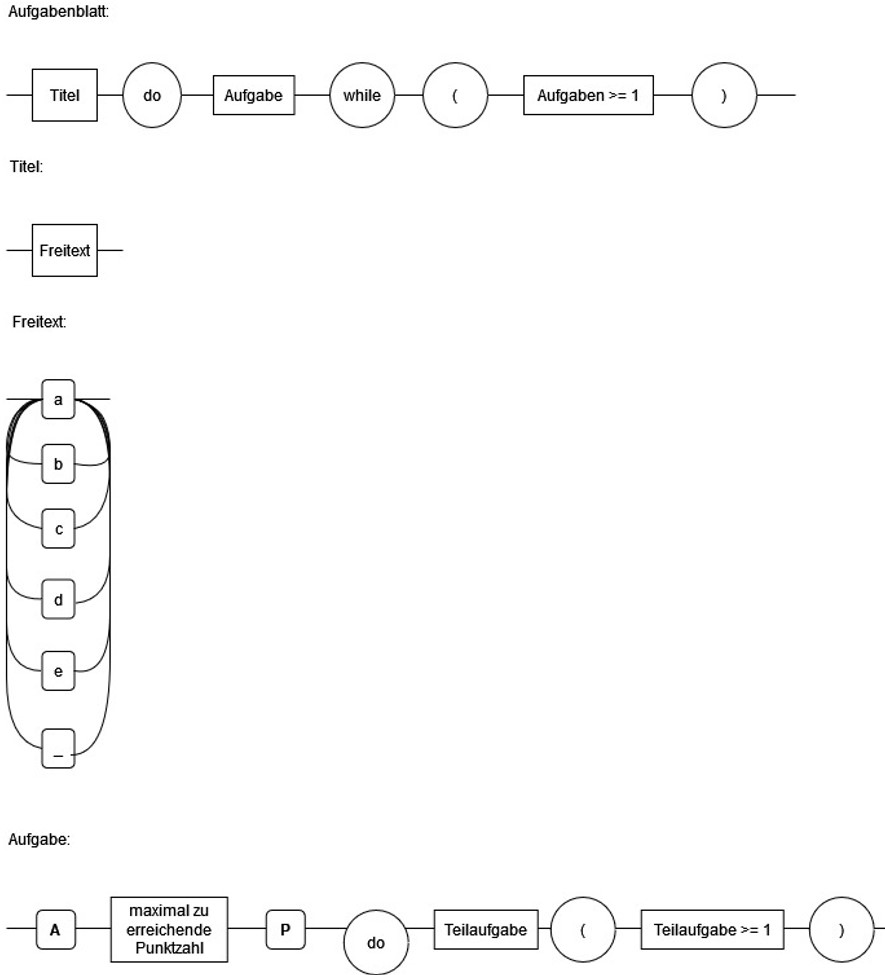
\includegraphics[width=15 cm]{syntax1.jpg}
  \end{center}

  \begin{center}
    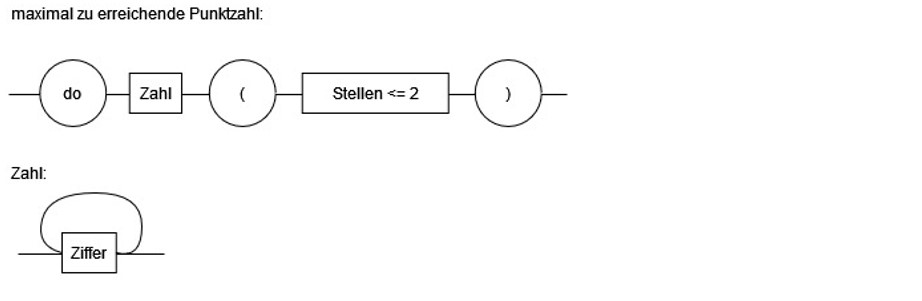
\includegraphics[width=15 cm]{syntax2.jpg}
  \end{center}

  \begin{center}
    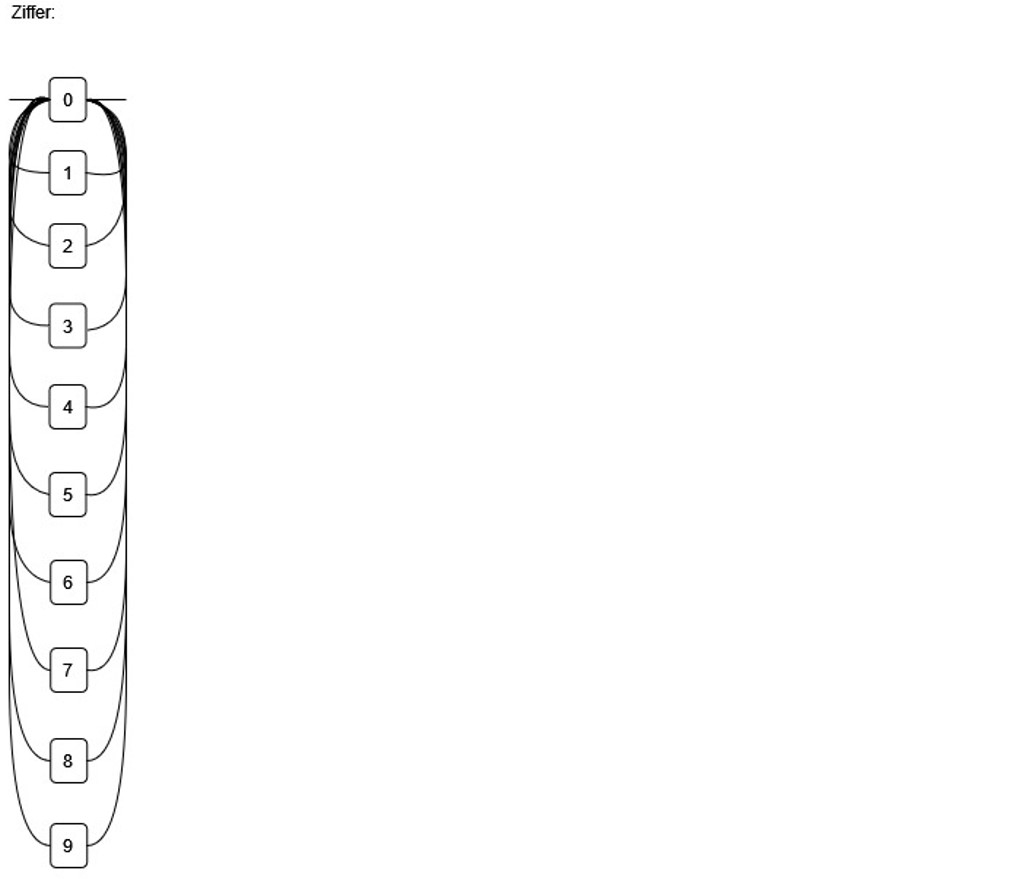
\includegraphics[width=15 cm]{syntax3.jpg}
  \end{center}

  \begin{center}
    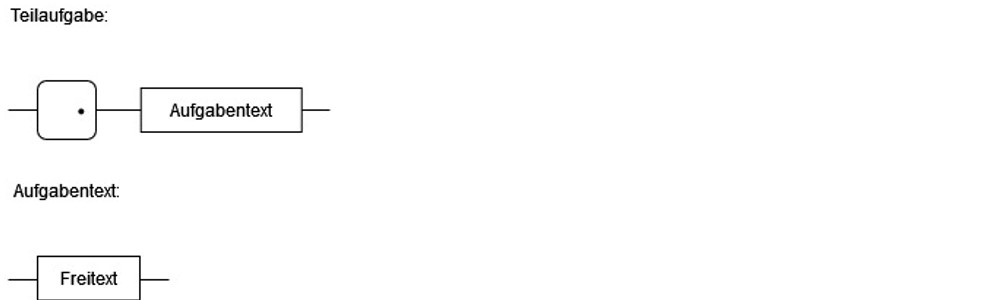
\includegraphics[width=15 cm]{syntax4.jpg}
  \end{center}

\end{itemize}

\newpage

\textbf{Aufgabe T8.2:} BNF (6 + 2 = 8 Punkte)

Nachfolgend sei eine Grammatik in Form der BNF gegeben:

\begin{center}
  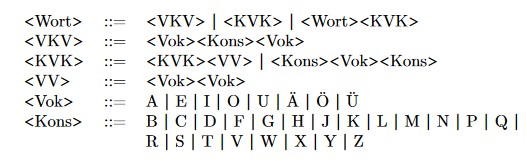
\includegraphics[width=10cm]{gramm.jpg}
\end{center}  
\begin{itemize}
  \item [(a)] Geben Sie für die folgenden Worte an, ob diese durch die gegebene BNF abgebildet werden und begründen Sie ihre Antwort:
  
\begin{itemize}
  \item [i)] LILIE

  Das Wort wird durch die Grammatik abgebildet, da LIL ein 
  \textless KVK\textgreater~ ist und IE ein \textless VV\textgreater. Daraus 
  lässt sich das zulässige \textless KVK\textgreater ::= \textless 
  KVK\textgreater \textless VV\textgreater ~bilden. Als \textless Wort\textgreater~  ist 
  ein \textless KVK\textgreater~ zulässig.

  \item [ii)] ZUCKER
  
  Das Wort wird durch die Grammatik abgebildet, da ZUC ein 
  \textless KVK\textgreater ~ist. Ein \textless KVK\textgreater~ ist ein 
  zulässiges \textless Wort\textgreater~. KER ist ebenfalls ein
  \textless KVK\textgreater~ die Konkatenation von ZUC und KER biltet ein 
  Zulässiges \textless Wort\textgreater~ wegen 
  \textless Wort\textgreater~ ::= \textless Wort\textgreater~ \textless KVK\textgreater.

  \item [iii)] AUBERGINE
  
  Das Wort wird nicht durch die Grammatik abgebildet, da AU ein 
  \textless VV\textgreater~ ist und BER ein \textless KVK\textgreater. 
  Es gibt keine Regel laut der auf ein \textless VV\textgreater~ ein \textless KVK\textgreater folgen darf.

  \item [ iv)] BITTERMANDEL
  
  Das Wort wird durch die Grammatik abgebildet, da BIT, TER, MAN, DEL alles 
  \textless KVK\textgreater's sind und nach
  \textless Wort\textgreater~ ::= \textless Wort\textgreater~ \textless KVK\textgreater
  ergeben konkatenierte \textless KVK\textgreater's ein zulässiges \textless Wort\textgreater.

  \item [v)] BASILIKUM
  
  Das Wort wird nicht durch die Grammatik abgebildet, da BAS ein
  \textless KVK\textgreater~ ist und ILI ein \textless VKV\textgreater. 
  In der Grammatik existert keine gültige Regel in der ein 
  \textless VKV\textgreater~ auf ein \textless KVK\textgreater~ folgen darf.

  \item [vi)] BLAUBEERE
  
  Das Wort wird nicht durch die Grammatik abgebildet, da  B ein 
  \textless Kons\textgreater~ und L ein \textless Kons\textgreater~ ist.
  In der Grammatik existert keine gültige Regel in der ein 
  \textless Kons\textgreater~ auf ein \textless Kons\textgreater~ folgen darf.


\end{itemize}

\newpage

  \item [(b)] Nennen Sie zwei deutsche Wörter, jeweils bestehend aus 5 oder mehr Buchstaben, die durch die gegebene BNF gebildet werden können. Dabei müssen die beiden Wörter in gängigen Wörterbüchern zu finden sein. Zusammengesetzte Worte sind dabei auch erlaubt.
  
  \begin{itemize}
    \item KACHEL
    \item TACKER
  \end{itemize}
\end{itemize}

\newpage

\textbf{Aufgabe T8.3:} Code-Verständnis (1 Punkte)

Ihnen wird die Datei \textit{HelloJava.java} bereitgestellt. Der Code beinhaltet ein vollständiges Programm, das allerdings einige Funktionen nutzt, die Sie bisher noch nicht kennengelernt haben.

Kopieren Sie den Code oder nutzen Sie die gegebene Datei und führen Sie diese aus. (Sie können beispielsweise die in der Vorlesung vorgestellte Software Eclipse nutzen.) Beschreiben Sie in knappen Sätzen, was die Aufgabe des Programms ist und welche Eingaben wie verwertet werden.

Das Programm berechnet alle Primzahlen bis zum eingegebenen Wert n. Als Eingaben werden ganzzahlige, positve und negative
Integer aktzeptiert. Characters und Floatingpoints führen zum Programabsturz. Bei
$n \le 1$ werden keine Primzahlen zurückgegeben, da die kleinstmögliche Primzahl 2 ist
und Primzahlen nur im positiven definiert sind. Das Ergebnis ist folglich korrekt und 
der Programm wird vollständig ausgeführt.

\newpage

\textbf{Aufgabe T8.4:} While / Do While / For Schleife $(2+2+2=6$ Punkte) 

In der Vorlesung haben Sie verschiedene Schleifen kennengelernt. Nun geben Sie ein Programm in Auftrag, das den Satz \mintinline{Java}{"Hallo Welt"} $n$ mal ausgibt und dafür eine Schleife verwendet. Dabei kann $n$ Werte im Interval $I=[0, \infty)$ annehmen. Ihnen wurden nun drei verschiedene Programme geschickt, die sich jeweils einer Art von Schleife bedienen. Da Sie sich noch nicht sicher sind, welche Art von Schleife Ihnen am besten gefällt, wollen Sie die Möglichkeit haben, zwischen den verschiedenen Formen zu wechseln. Beschreiben Sie daher für Schleifen mit $n$ Iterationen,

\begin{itemize}

  \item [] Jede der drei Schleifen benötigt einen Parameter \mintinline{Java}{n}, der der Methode 
  übergeben wird. Der Parameter gibt an, wie oft die Schleife durchlaufen werden 
  soll. Desweiteren ist es sinnvoll eine Laufvariable zu definieren, welche auf 0
  initialisiert wird. Diese Variable ist zwar nicht für alle Schleifentypen 
  erforderlich, erleichtert jedoch die Umwandlung von einen zum anderen Typ.

  \item [(a)] wie eine \mintinline{Java}{while} in eine \mintinline{Java}{do while} Schleife umgewandelt werden kann und umgekehrt,

  Für ein \mintinline{Java}{while}-Programm würde zu Beginn der Methode eine 
  Variable \mintinline{Java}{i} vom Typen \mintinline{Java}{int} auf 0 initialisiert werden. Im Schleifenkopf steht die
  Bedingung, wie lange der Schleifenrumpf ausgeführt werden soll. In diesem Falle 
  wäre \mintinline{Java}{while (n>i)} eine sinnvolle Möglichkeit. Darauf folgt der
  Schleifenrumpf, in dem der Befehl \mintinline{Java}{System.out.println"Hello World!";} zur Ausgabe des 
  \mintinline{Java}{String} \mintinline{Java}{"Hello World!"} gefolgt 
  von der Inkrementierung der Laufvariable \mintinline{Java}{i} durch \mintinline{Java}{i++;} folgt.

  Um das oben beschriebene \mintinline{Java}{while}-Programm in ein \mintinline{Java}{do while}-Programm zu
  überführen, würde der Schleifenkopf mit einem \mintinline{Java}{do} beginnen. Der Schleifenrumpf ist
  identisch mit dem des \mintinline{Java}{while}-Programms. Auf den Schleifenrumpf folgt die
  Abbruchbedingung, welche identisch ist mit der Bedingung des \mintinline{Java}{while}-Programms,
  also \mintinline{Java}{while (n>i)}.

  Der Unterschied zwischen einer \mintinline{Java}{while} in einer \mintinline{Java}{do while} Schleifen
  besteht darin, dass bei einer \mintinline{Java}{while} Schleife der Schleifenrumpf
  solange ausgeführt wird, wie die Schleigenbedingung wahr ist. Bei einer \mintinline{Java}{do while} Schleife
  wird der Schleifenrumpf mindestens einmal ausgeführt und danach solange, wie 
  die Schleifenbedingung wahr ist.

  Die Umgekehr von einer \mintinline{Java}{do while}-Schleife in eine \mintinline{Java}{while}-Schleife
  erfolgt analog zu dem oben beschriebenen Weg, da die Umwanldungsschritte äquivalent sind. 
  Dazu wird das \mintinline{Java}{do} ersetzt durch die Schleifenbedingung \mintinline{Java}{while (n>1);}
  und das \mintinline{Java}{while (n>1);} am Ende der \mintinline{Java}{do while}-Schleife entfernt.

  \newpage

  Zur Veranschaulichung folgt der entsprechende Java-Code:
  \begin{itemize}
    \item [] \inputminted[]{Java}{A8_4_while_do_while.java}
  \end{itemize}

  \item [(b)] wie eine \mintinline{Java}{while} in eine \mintinline{Java}{for} Schleife umgewandelt werden kann und umgekehrt und

  Das in Aufgabenteil a) beschriebene \mintinline{Java}{while}-Programm, lässt sich wie folgt in 
  ein \mintinline{Java}{for}-Programm umwandeln. Die Laufvariable \mintinline{Java}{int i = 0;} wird nun im Schleifenkopf
  der \mintinline{Java}{for}-Schleife initialisiert, darauf folgt die Schleifenbedingung mit \mintinline{Java}{i<n;} und dann die 
  Inkrementierung von \mintinline{Java}{i} mit \mintinline{Java}{i++}. Bei der \mintinline{Java}{for}-Schleife
  befindet sich im Schleifenrumpf nur der Befehl \mintinline{Java}{System.out.println"Hello World!";},
  da die Inkrementierung bereits im Kopf stattfindet.

  Zur Umwandlung der \mintinline{Java}{for}-Schleife in eine \mintinline{Java}{while}-Schleife wird die
  Laufvariable \mintinline{Java}{int i = 0;} aus dem Schleifenkopf entfernt und vor der
  Schleife initialisiert. Die Inkrementierung von \mintinline{Java}{i} durch \mintinline{Java}{i++;}
  wird aus dem Schleifenkopf entfernt und in den Schleifenrumpf eingfügt.

  Zur Veranschaulichung folgt der entsprechende Java-Code:
  \begin{itemize}
    \item [] \inputminted[]{Java}{A8_4_for.java}
  \end{itemize}

  \item [(c)] wie eine \mintinline{Java}{do while} in eine \mintinline{Java}{for} Schleife umgewandelt werden kann und umgekehrt.
  
  Zur Umwandlung des in Aufgabenteil a) beschriebenen \mintinline{Java}{do while}-Programms 
  in ein \mintinline{Java}{for}-Programm wird das \mintinline{Java}{do} ersetzt durch ein \mintinline{Java}{for} gefolgt von
  einer runden Klammer. Die Initialisierung der Laufvariable \mintinline{Java}{int i = 0;} wird 
  vor der \mintinline{Java}{do while}-Schleife entfernt und nach der runden
  Klammer eingefügt. Die Schleifenbedingung am Ende der \mintinline{Java}{do while}-Schleife
  \mintinline{Java}{while (n>i);} wird entfernt und nach der Laufvariable im Schleifenkopf als
  \mintinline{Java}{i<n;} eingefügt. Die Inkrementierung \mintinline{Java}{i++;} wird aus dem
  Schleifenrumpf entfernt und nach der Schleifenbedingung im Schleifenkopf der \mintinline{Java}{for}-Schleife
  eingefügt. Der Schleifenkopf wird durch eine runde Klammer geschlossen. In
  geschwungenen Klammern folgt der Schleifenrumpf mit \mintinline{Java}{System.out.println("Hello World!");}

  Die Umwandlung der \mintinline{Java}{for}-Schleife in eine \mintinline{Java}{do while}-Schleife erfolgt wieder analog.
  Der Schleifenkopf der \mintinline{Java}{for}-Schleife, also \mintinline{Java}{for(int i = 0; i < n; i++)} wird
  durch \mintinline{Java}{do} ersetzt. Die Laufvariable \mintinline{Java}{int i = 0;} wird
  vor der Schleife initialisiert. Im Schleifenrumpf wird die Inkrementierung \mintinline{Java}{i++;} eingefügt. 
  am Ende der Schleife wird die Schleigenbedingung \mintinline{Java}{while(n>i)} eingefügt.
  
  Zur Veranschaulichung folgt der entsprechende Java-Code:
  \begin{itemize}
    \item [] \inputminted[]{Java}{A8_4_do_while.java}
  \end{itemize}

\end{itemize}

Bitte beachten Sie, dass Ihre Beschreibung allgemein gültig und für alle möglichen $n \in I$ gelten soll. Sie dürfen allerdings für Ihre Erklärungen das oben genannte Beispiel nutzen.

\newpage

\textbf{Aufgabe T8.5:} Nikolaus 1 (3 Bonuspunkte)

Der Nikolaus ist auf der Suche nach Cartoons, die die Themen Informatik und Weihnachten verbinden. Reichen Sie einen solchen Cartoon (entweder selbst gezeichnet oder mit Quellenangabe!) ein und erklären Sie kurz, d.h. in maximal 3 Sätzen, warum dieser Cartoon einen Bezug zur Informatik hat und wie ein Bezug zu den bisher behandelten Themen in der Vorlesung Informatik 1 besteht. Wenn keine Erklärung angegeben wird, gibt es nur 1 Punkt und falls kein Bezug zur Vorlesung erklärt wird, gibt es nur 2 Punkte.

\begin{center}
  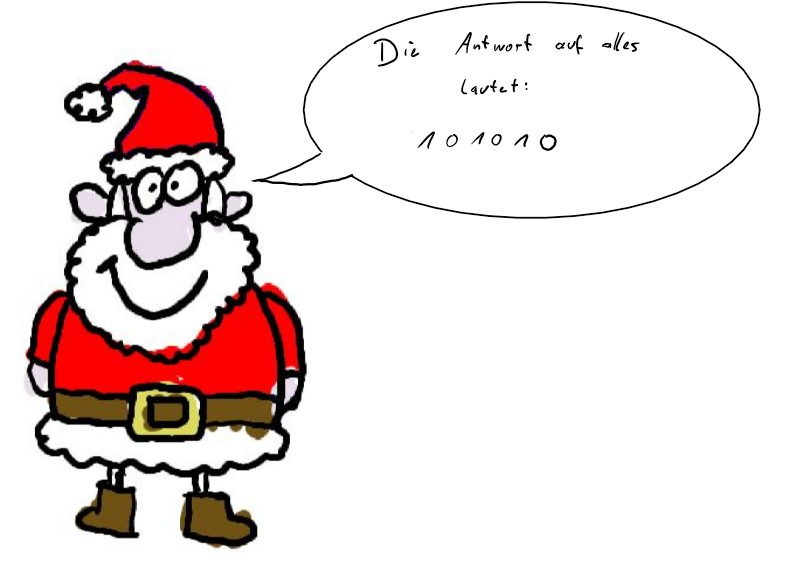
\includegraphics[width=15cm]{witz.jpg}
\end{center}

101010 binär ist 42 dezimal. Binärumrechnungen wurden in der Vorlesung behandelt und sind ein grundlegendes Element in der Informatik. 101010 war das Passwort zum Learnweb-Kurs. Warum das für Prof. Linsens Humor spricht muss ich 

\newpage

\textbf{Aufgabe P8.6:} Nikolaus 2 (4 Punkte $+3$ Bonuspunkte)

Für die diesjährige Nikolausaufgabe hat Ihr Übungsleiter einen Nikolaus gemalt. Leider gab es vorher auf dem Weihnachtsmarkt ein oder zwei Gläser Eierlikör zu viel, sodass ihm dabei ein Fehler unterlaufen ist. Gegeben ist das Programm MakeNikolaus.java, dass das ebenfalls gegebene Bild Nikolaus.jpg einlädt und als multidimensionales Array zur Verfügung stellt. Im Array sind die RGB-Farbwerte der Pixel gespeichert und die Dimensionen des Arrays entsprechen jeweils der Höhe und der Breite des Bildes. Eine genaue Beschreibung finden Sie im Sourcecode. Außerdem wandelt das Programm das Array wieder in ein Bild um und speichert es als NewNikolaus.jpg.
\begin{itemize}
  \item [(a)] Passen Sie die Variable String path an, sodass das Ihnen bereitgestellte Bild Nikolaus.jpg geladen wird und testen Sie, ob es unverändert als NewNikolaus.jpg im selben Ordner gespeichert wird. Fügen Sie nun im Quelltext an angegebener Stelle Ihren Code hinzu, der das multidimensionale Array durchläuft und somit den Wert jedes Pixels ausliest. Dabei handelt es sich um einen einzelnen Integer Wert. Nutzen Sie die bereitgestellte Funktion isBlue, um zu überprüfen, ob es sich um ein blaues Pixel handelt. Sollte dieser Fall eintreffen, ersetzen Sie den Wert im multidimensionalen Array mit einem roten Pixel. Nutzen Sie hierfür die bereitgestellte Funktion makeColor(int $r$, int $g$, int $b$ ) mit den Werten $r=255, g=0, b=0$. Das fertige Ergebnis sollte etwa so aussehen:

  \begin{center}
  
\includegraphics[width=3cm]{2022_12_05_3f6eb410f05a7976cd28g-3}
  \end{center}
  
  \item [(b)] (Bonus) Passen Sie den Code in a) so an, dass die Mütze mehrfarbig ist, z.B. mit einen Farbverlauf oder einem Muster. Dabei können Sie so kreativ sein, wie Sie möchten. Die Lösung für Aufgabenteil a) dürfen Sie dafür auskommentieren.
  
  \begin{center}
    
\includegraphics[width=3cm]{NewNikolaus.jpg}
    \end{center}

\end{itemize}

\newpage

\begin{itemize}
  \item [] \inputminted[]{Java}{MakeNikolaus.java}
\end{itemize}

\end{document}